\section{Configuração no ESP32}

Para a realização da prática, usamos um ESP32 de 30 pinos, uma protoboard de 400 pontos, um potenciômetro, um LED RGB por falta de um LED simples, um resistor de 390 \textit{ohms}, cinco cabos macho-fêmea e um cabo serial micro-USB.

\begin{figure}[H]
    \centering
    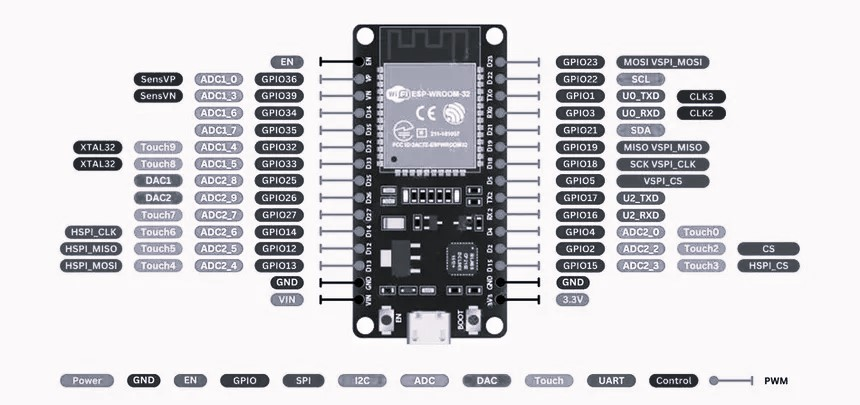
\includegraphics[width=0.5\linewidth]{img/esp32_pinout.png}
    \caption{Pinout do ESP32.}
    \label{fig:esp32-pinout}
\end{figure}

Colocamos os terminais do potenciômetro na protoboard para não utilizar cabos. O potenciômetro possui três terminais: VCC, \textit{output} e GND. Conectamos o terminal VCC ao pino VCC do ESP32 utilizando um cabo macho-fêmea. Fizemos o mesmo com o GND. 

\begin{figure}[H]
    \centering
    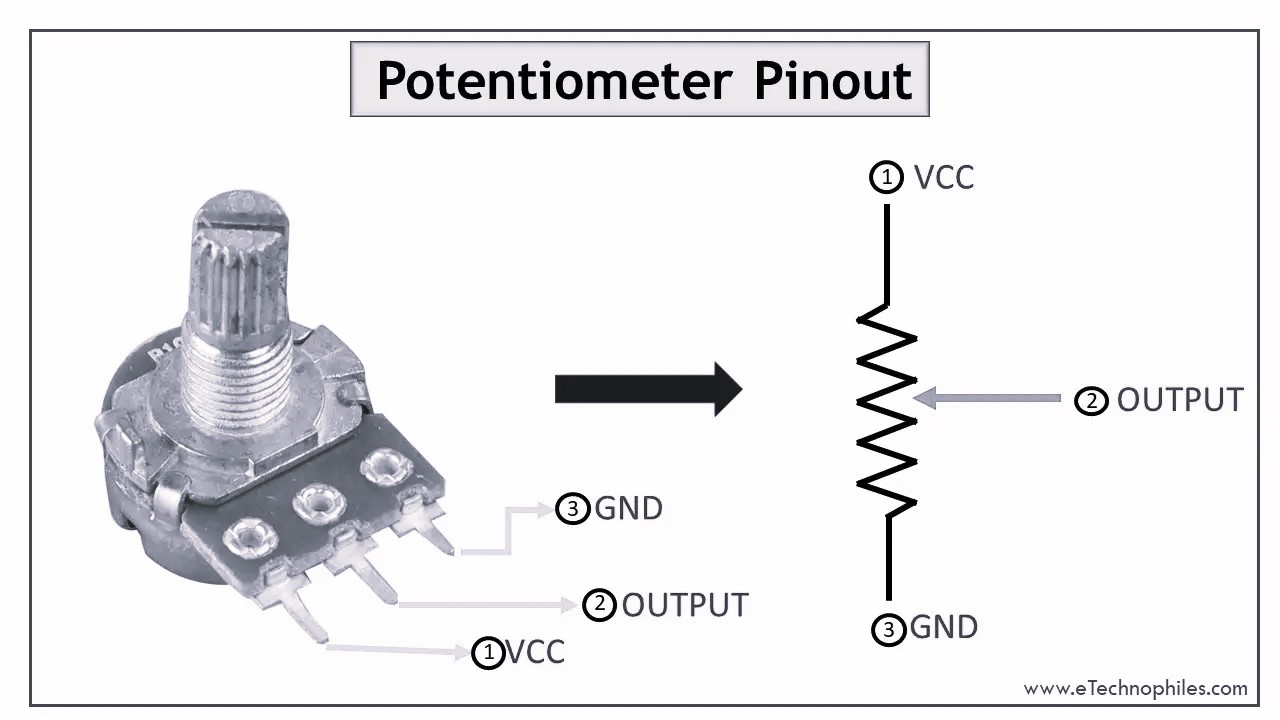
\includegraphics[width=0.5\linewidth]{img/Pot-pinout.jpg}
    \caption{Pinout do potenciômetro.}
    \label{fig:pot-pinout}
\end{figure}

Já o terminal \textit{output} precisa ser conectado a um pino de entrada analógica (ADC) do ESP32. Conferindo o \textit{pinout}, descobrimos que todos os pinos de GPIO do lado do botão EN são de entrada analógica. Existem pinos ADC do outro do lado do ESP32, mas eles não funcionam quando o Wi-Fi está conectado, e precisamos dele. Escolhemos o pino 34.

Por último, colocamos o LED RGB na protoboard. Como é um projeto pequeno, ele pode ficar em qualquer lugar, pois há um pino de GND para ele, onde conectamos utilizando um cabo macho-fêmea. Só vamos usar um dos terminais, pois é o bastante para o teste. Escolhemos o terminal vermelho e colocamos o resistor na coluna antes de ligá-lo a um pino do ESP32, que dessa vez foi o pino 22.